% 2010 年浙江卷理科第 20 题：矩形 ABCD 沿 EF 翻折为 A'EF。
% 来源 PDF：普通高考/2010/2010浙江理.pdf，SHA-256 c61b26c8cab009d567644272afc34d81e3174ffa90244c333ecfb27d61034a00。
% 原页：第 2 页（A3 三栏）第 1 栏，书页码 640。
% 重绘依据：照原页透视，D 左下、C 右下、B 右上、A 左上（原位置），E 在 AB 上，
%   F 在 AD 上；A' 在平面 BEF 上方，A'E、A'F、EF 为实线，AE、AF 为虚线；
%   M 在 FD 上、N 在 BC 上，MN 为第二折痕。
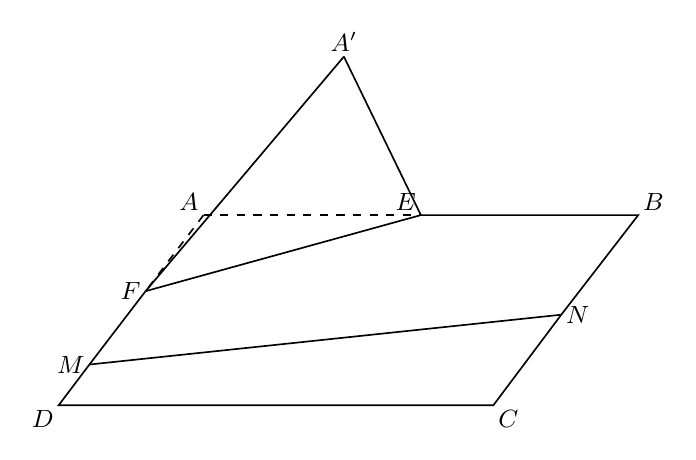
\begin{tikzpicture}[scale=1.15, semithick, every node/.style={inner sep=1.5pt, font=\small}]
  \coordinate (D) at (0,0);
  \coordinate (C) at (4.8,0);
  \coordinate (B) at (6.4,2.1);
  \coordinate (A) at (1.6,2.1);
  \coordinate (E) at (4.0,2.1);
  \coordinate (F) at (0.96,1.26);
  \coordinate (M) at (0.34,0.45);
  \coordinate (N) at (5.55,1.0);
  \coordinate (A1) at (3.15,3.85);

  % 矩形实线部分
  \draw (E) -- (B) -- (N) -- (C) -- (D) -- (M) -- (F);
  % 折痕 EF
  \draw (E) -- (F);
  % 翻折后的三角形
  \draw (A1) -- (E);
  \draw (A1) -- (F);
  % 原位置 A 的虚线
  \draw[dashed] (A) -- (E);
  \draw[dashed] (A) -- (F);
  % 第二折痕
  \draw (M) -- (N);

  \node[above] at (A1) {$A'$};
  \node[above left] at (A) {$A$};
  \node[above left] at (E) {$E$};
  \node[above right] at (B) {$B$};
  \node[left] at (F) {$F$};
  \node[left] at (M) {$M$};
  \node[right] at (N) {$N$};
  \node[below left] at (D) {$D$};
  \node[below right] at (C) {$C$};
\end{tikzpicture}
